\documentclass[14pt]{beamer}
\usepackage{./Estilos/BeamerUVM}
\usepackage{./Estilos/ColoresLatex}
\usetheme{Madrid}
\usecolortheme{default}
%\useoutertheme{default}
\setbeamercovered{invisible}
% or whatever (possibly just delete it)
\setbeamertemplate{section in toc}[sections numbered]
\setbeamertemplate{subsection in toc}[subsections numbered]
\setbeamertemplate{subsection in toc}{\leavevmode\leftskip=3.2em\rlap{\hskip-2em\inserttocsectionnumber.\inserttocsubsectionnumber}\inserttocsubsection\par}
% \setbeamercolor{section in toc}{fg=blue}
% \setbeamercolor{subsection in toc}{fg=blue}
% \setbeamercolor{frametitle}{fg=blue}
\setbeamertemplate{caption}[numbered]

\setbeamertemplate{footline}
\beamertemplatenavigationsymbolsempty
\setbeamertemplate{headline}{}


\makeatletter
% \setbeamercolor{section in foot}{bg=gray!30, fg=black!90!orange}
% \setbeamercolor{subsection in foot}{bg=blue!30}
% \setbeamercolor{date in foot}{bg=black}
\setbeamertemplate{footline}
{
  \leavevmode%
  \hbox{%
  \begin{beamercolorbox}[wd=.333333\paperwidth,ht=2.25ex,dp=1ex,center]{section in foot}%
    \usebeamerfont{section in foot} {\insertsection}
  \end{beamercolorbox}%
  \begin{beamercolorbox}[wd=.333333\paperwidth,ht=2.25ex,dp=1ex,center]{subsection in foot}%
    \usebeamerfont{subsection in foot}  \insertsubsection
  \end{beamercolorbox}%
  \begin{beamercolorbox}[wd=.333333\paperwidth,ht=2.25ex,dp=1ex,right]{date in head/foot}%
    \usebeamerfont{date in head/foot} \insertshortdate{} \hspace*{2em}
    \insertframenumber{} / \inserttotalframenumber \hspace*{2ex} 
  \end{beamercolorbox}}%
  \vskip0pt%
}
\makeatother

\makeatletter
\patchcmd{\beamer@sectionintoc}{\vskip1.5em}{\vskip0.8em}{}{}
\makeatother

% \usefonttheme{serif}
\usepackage[clock]{ifsym}

\sisetup{per-mode=symbol}
\resetcounteronoverlays{saveenumi}

\title{\Large{Presentación syllabus - Laboratorio} \\ \normalsize{Física III}}
\date{30 de agosto de 2023}

\begin{document}
\maketitle

\section*{Contenido}
\frame{\frametitle{Contenido} \tableofcontents[currentsection, hideallsubsections]}

% \section{Objetivos}
% \frame{\tableofcontents[currentsection, hideothersubsections]}
% \subsection{Metas esperadas}

% \begin{frame}
% \frametitle{Objetivos del curso}
% \setbeamercolor{item projected}{bg=bananayellow,fg=ao}
% \setbeamertemplate{enumerate items}{%
% \usebeamercolor[bg]{item projected}%
% \raisebox{1.5pt}{\colorbox{bg}{\color{fg}\footnotesize\insertenumlabel}}%
% }
% \begin{enumerate}[<+->]
% \item El alumno desarrollará algunas habilidades propias de la investigación como la creación de modelos a través de la observación, la formulación de hipótesis, el manejo de variables, etc., \pause para comprender, interpretar y analizar fenómenos físicos que resultan fundamentales en la comprensión de su entorno.
% \seti
% \end{enumerate}
% \end{frame}
% \begin{frame}
% \frametitle{Objetivos del curso}
% \setbeamercolor{item projected}{bg=bananayellow,fg=ao}
% \setbeamertemplate{enumerate items}{%
% \usebeamercolor[bg]{item projected}%
% \raisebox{1.5pt}{\colorbox{bg}{\color{fg}\footnotesize\insertenumlabel}}%
% }
% \begin{enumerate}[<+->]    
% \conti
% \item Asimismo, se espera que al analizar las aportaciones de la física en diferentes ámbitos, el alumno logre comprender los retos y problemas de su entorno, así como las diversas formas que existen para resolverlos.
% \seti
% \end{enumerate}
% \end{frame}
% \begin{frame}
% \frametitle{Objetivos del curso}
% Con la conciencia de que de los desarrollos científicos y tecnológicos surgen implicaciones sociales que obligan a tomar decisiones que se deben analizar para emitir juicios y actuar de manera responsable.
% \end{frame}
% \begin{frame}
% \frametitle{Objetivos del curso}
% \setbeamercolor{item projected}{bg=bananayellow,fg=ao}
% \setbeamertemplate{enumerate items}{%
% \usebeamercolor[bg]{item projected}%
% \raisebox{1.5pt}{\colorbox{bg}{\color{fg}\footnotesize\insertenumlabel}}%
% }
% \begin{enumerate}[<+->]    
% \conti
% \item Finalmente, se espera que el alumno valore el trabajo colaborativo para el logro de metas y respete las opiniones de los demás como vía de enriquecimiento de ideas y fomento a la tolerancia.
% \end{enumerate}
% \end{frame}

\section{Evaluación}
\frame{\tableofcontents[currentsection, hideothersubsections]}
\subsection{Esquema de evaluación}

\begin{frame}
\frametitle{Trabajo en el Laboratorio}
El trabajo en Laboratorio consistirá en el montaje de prácticas dirigidas en las sesiones de clase.
\end{frame}
\begin{frame}
\frametitle{Etapas de trabajo}
\setbeamercolor{item projected}{bg=aquamarine,fg=black}
\setbeamertemplate{enumerate items}{%
\usebeamercolor[bg]{item projected}%
\raisebox{1.5pt}{\colorbox{bg}{\color{fg}\footnotesize\insertenumlabel}}%
}
\begin{enumerate}[<+->]
\item Discusión de la práctica.
\item Montaje experimental.
\item Interpretación de resultados y reporte.
\end{enumerate}
\end{frame}
\begin{frame}
\frametitle{Discusión de la práctica}
Durante el año escolar se realizarán varias prácticas, en una primera sesión se discutirá sobre el objetivo de la misma, así como el marco teórico para su comprensión.
\end{frame}
\begin{frame}
\frametitle{Discusión de la práctica}
El alumno deberá de complementar la revisión durante la semana, de tal manera que en la clase de montaje, tendrá el soporte de conocimiento necesario para realizar la práctica.
\end{frame}
\begin{frame}
\frametitle{Montaje de la práctica}
En una segunda sesión se realizará el montaje de la práctica durante la clase, esto implica trabajo en equipo.
\end{frame}
\begin{frame}
\frametitle{Recabando datos e información}
Cada equipo de trabajo, deberá de recolectar los datos de la práctica, de tal manera que con trabajo adicional durante la semana, llegará a la siguiente sesión con un trabajo preliminar.
\end{frame}
\begin{frame}
\frametitle{Interpretación de datos y reporte}
En la tercera sesión, cada equipo de trabajo revisará los resultados preliminares, discutirán sobre los hechos hallados y revisarán su congruencia con el marco téorico.
\end{frame}
\begin{frame}
\frametitle{Elaboración del reporte}
Una vez revisada la parte de interpretación, cada alumno realizará un reporte de la práctica.
\\
\bigskip
\pause
Se dispondrá de una rúbrica para la evaluación del reporte de la práctica.
\end{frame}
\begin{frame}
\frametitle{Reporte individual}
Aunque el trabajo se realizará en equipo, el reporte debe de ser INDIVIDUAL.
\end{frame}
\begin{frame}
\frametitle{Reporte individual}
Se busca que cada alumna(o) desarrolle habilidades y compentencias de análisis, interpretación y escritura de resultados.
\end{frame}
\begin{frame}
\frametitle{Calificación de Laboratorio}
El peso de la calificación de Laboratorio corresponde al $30 \%$ de la calificación de cada examen parcial.
\\
\bigskip
\pause
Se tendrán cuatro exámenes parciales durante el ciclo escolar.
\end{frame}

\section{Temas para las prácticas}
\frame{\tableofcontents[currentsection, hideothersubsections]}
\subsection{Mecánica clásica}

\begin{frame}
\frametitle{Prácticas de movimiento}
Como primer tema para el trabajo en Laboratorio, se realizarán prácticas correspondientes al tema de mecánica clásica:
\end{frame}
\begin{frame}
\frametitle{Prácticas de movimiento}
\setbeamercolor{item projected}{bg=darkred,fg=white}
\setbeamertemplate{enumerate items}{%
\usebeamercolor[bg]{item projected}%
\raisebox{1.5pt}{\colorbox{bg}{\color{fg}\footnotesize\insertenumlabel}}%
}
\begin{enumerate}[<+->]
\item Movimiento rectilíneo uniforme.
\item Movimiento circular.
\item Leyes de Newton.
\end{enumerate}
\end{frame}

\subsection{Calor y energía}

\begin{frame}
\frametitle{Prácticas para la segunda parte}
Como tema para la segunda parte del curso, se revisarán actividades de calor, temperatura, electricidad y energía.
\end{frame}
\begin{frame}
\frametitle{Prácticas para la segunda parte}
\setbeamercolor{item projected}{bg=darkscarlet,fg=white}
\setbeamertemplate{enumerate items}{%
\usebeamercolor[bg]{item projected}%
\raisebox{1.5pt}{\colorbox{bg}{\color{fg}\footnotesize\insertenumlabel}}%
}
\begin{enumerate}[<+->]
\item Ley de Faraday.
\item Calor específico.
\item Transformación de energía.
\end{enumerate}
\end{frame}

% \section{Rúbrica de evaluación}
% \frame{\tableofcontents[currentsection, hideothersubsections]}
% \subsection{Componentes y nivel de desempeño}

% \begin{frame}
% \frametitle{Preparación - Excelente (2 puntos)}
% \begin{itemize}
% \item Identifica todas las variables del experimento, plantea sus objetivos.
% \item Buen proceso de preparación, muestra profundidad en la investigación del tema.
% \item Incluye las referencias bibliográficas.
% \end{itemize}
% \end{frame}
% \begin{frame}
% \frametitle{Preparación - Aceptable (1 puntos)}
% \begin{itemize}
% \item Identifica algunas de las variables del experimento.
% \item Cumplido en la preparación demuestra conocimiento del tema.
% \end{itemize}
% \end{frame}
% \begin{frame}
% \frametitle{Preparación - Insuficiente (0 puntos)}
% No identifica las variables del experimento, necesita mucha revisión para la tarea encargada.
% \end{frame}


% 2. Trabajo experimental
% • Logra conectar su investigación en diferentes aspectos de la práctica.
% • Desarrolla la práctica experimental de manera adecuada siguiendo los pasos correctamente.
% • Toma en cuenta la mayor par- te de las instrucciones.
% • Requiere ayuda para desarrollar el trabajo experimental
% • No sigue correctamente las instrucciones, desatiende al desarrollar el trabajo experimental.
% 3. Participación
% • Su participación es pertinente y activa, es fundamental para la ejecución del experimento y el buen desarrollo de cada uno de los conceptos.
% • Su participación es oportuna, aporta buenos elementos y presta atención a las diferentes participaciones
% • Su participación es oportuna, aporta buenos elementos y presta atención a las diferentes participaciones
% • Está presente pero presta poca atención a las distintas instrucciones para la ejecución
% de la práctica.
% 4. Reporte de Resultados
% • Interpreta correctamente los resultados del experimento.
% • Presenta los datos en forma profesional demostrando un nivel alto de comprensión sobre el contenido.
% • Interpreta con algunos erro- res los resultados del experimento, tiene errores en los cálculos, requiere de alguna revisión para alcanzar el nivel de excelente.
% • Interpreta erróneamente los resultados, comete muchos errores en los cálculos.
% • La presentación de los datos es confusa el trabajo no merece crédito.
% 5. Elaboración de Conclusiones
% • Elabora conclusiones válidas, bien fundamentadas basadas en el correcto análisis de la experimentación.
% • Justifica que los explícita- mente que los objetivos se hayan alcanzado o no.
% • Elabora conclusiones parcial- mente válidas, basadas en una interpretación en parte correcta de los resultados
% • Menciona vagamente el logro de los objetivos
% • Elabora conclusiones no válidas, basadas en una interpretación deficiente de los resultados.
% • No menciona en logro de objetivos, no llega a ninguna conclusión.


\section{Trabajo en Laboratorio}
\frame{\tableofcontents[currentsection, hideothersubsections]}

\subsection{Asistencia}

\begin{frame}
\frametitle{Pase de asistencia}
Se realizará el \textocolor{red}{pase de asistencia} luego de la tolerancia para ingresar a la clase, que es de 5 minutos.
\end{frame}
\begin{frame}
\frametitle{Pase de asistencia}
En caso de que la(el) alumna(o) no se encuentre en la clase al momento del pase de asistencia, se le marcará como inasistencia, así haya ingresado luego de completar el pase.
\end{frame}
\begin{frame}
\frametitle{De la asistencia}
La sesión de Laboratorio se lleva a cabo una vez a la semana.
\\
\bigskip
\pause
Siendo indispensable asistir a cada una de las clases de Laboratorio.
\end{frame}
    
\subsection{Elementos necesarios}

\begin{frame}
\frametitle{Elementos necesarios}
Para el trabajo en laboratorio, es necesario utilizar una BATA BLANCA.
\\
\bigskip
\pause
Revisaremos que en el Manual de Seguridad y Normas de Higiene el Laboratorio, el uso de Bata es requisito.
\end{frame}
\begin{frame}
\frametitle{¿Qué pasa si no traigo la bata?}
En caso de que no se tenga la bata, la(el) alumna(o) no podrá permanecer en el Laboratorio, \pause se notificará a la Coordinación Académica para que los acompañe a la Biblioteca en donde tendrán que realizar una actividad entregable al concluir la clase.
\end{frame}
\begin{frame}
\frametitle{¿Qué pasa si no traigo la bata?}
Deberán de completar la actividad, pero no podrán reponer la actividad de Laboratorio y contarán con inasistencia.
\\
\bigskip
\pause
Es recomendable que se prevengan para contar con una bata blanca.
\end{frame}
\begin{frame}
\frametitle{¿Qué pasa si falto a una clase?}
En caso de una inasistencia, la calificación de la práctica disminuye ya que en cada sesión se evalúa un componente.
\end{frame}
\begin{frame}
\frametitle{¿Qué pasa si falto a una clase?}
Si la falta es en la clase de montaje experimental, la alumna/alumno no podrá presentar los datos o resultados que obtuvieron sus compañeros de equipo.
\end{frame}
\begin{frame}
\frametitle{No se podrá reponer la actividades}
Recordemos nuevamente que solo se tendrá una sesión por semana, por lo que no se puede reponer la actividad en la que se no se asistió a clase.
\end{frame}

\begin{frame}
\frametitle{El Reglamento}
Revisaremos en la siguiente sesión el Manual de Seguridad y las Normas de Higiene para el Laboratorio.
\end{frame}

% \subsection{Primera actividad}

% \begin{frame}
% \frametitle{Primera actividad}
% Será necesario que cada alumno incluya en su cuardeno, carpeta de notas, etc. la \textocolor{ao}{síntesis de la asignatura}, con la firma del alumno así como del Tutor.
% \end{frame}
% \begin{frame}
% \frametitle{Primera actividad}
% De esta manera, se tendrá la claridad en el trabajo, la didáctica en la clase, el reglamento y las actividades a realizar durante el año escolar.
% \end{frame}
% \begin{frame}
% \frametitle{Actividad que cuenta}
% El presentar la síntesis de la asignatura debidamente firmada, contará en el puntaje de evaluación para el Laboratorio.
% \end{frame}
% \begin{frame}
% \frametitle{Entrega de la actividad}
% Se abrirá una asignación en Teams para el envío de una foto de la síntesis firmada por el alumno y el Tutor, además de tenerla en su cuaderno de trabajo.
% \end{frame}
% \begin{frame}
% \frametitle{Primeras actividades}
% Se informa al grupo que se está acabando de afinar el espacio de Laboratorio para las clases, \pause por lo que las primeras tres actividades se llevarán a cabo en el aula.
% \end{frame}
% \begin{frame}
% \frametitle{Primeras actividades}
% Estas primeras actividades contabilizarán como prácticas y por lo tanto, sumarán puntos para el primer examen parcial.
% \end{frame}
% \begin{frame}
% \frametitle{Consideración importante}
% Como ya se mencionó, se tendrá una clase de Laboratorio a la semana.
% \\
% \bigskip
% \pause
% No asistir a una clase compromete la evaluación, ya que no se podrá reponer la actividad a la que se haya asistido.
% \end{frame}

\section{Actividad}
\frame{\tableofcontents[currentsection, hideothersubsections]}
\subsection{Para la siguiente clase}

\begin{frame}
\frametitle{Actividad a realizar}
Se te pide que leas el \textocolor{cobalt}{Reglamento General para Laboratorios}, que se dejará en Teams.
\end{frame}
\begin{frame}
\frametitle{Actividad a realizar}
\begin{figure}
\centering
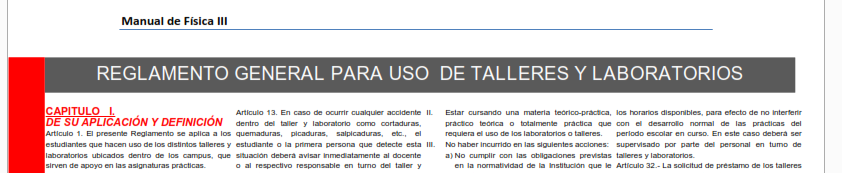
\includegraphics[scale=0.7]{Imagenes/Reglamento_01.png}
\end{figure}
\end{frame}
\begin{frame}
\frametitle{Actividad a realizar}
\begin{figure}
\centering
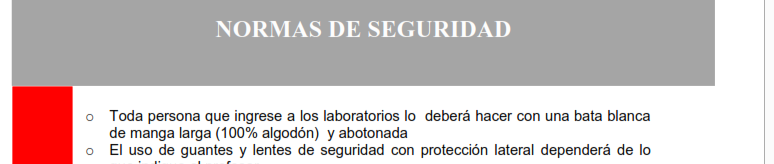
\includegraphics[scale=0.7]{Imagenes/Reglamento_02.png}
\end{figure}
\end{frame}
\begin{frame}
\frametitle{Actividad para la siguiente clase}
En la siguiente clase haremos una dinámica para revisar el Reglamento, por lo que la lectura previa será necesaria.
\end{frame}
\end{document}